%----------------------------------------------------------------------------------------
%	PACKAGES
%----------------------------------------------------------------------------------------

\documentclass[paper=a4, fontsize=11pt]{scrartcl} % A4 paper and 11pt font size
\usepackage{fourier} % Use the Adobe Utopia font for the document - comment this line to return to the LaTeX default
\usepackage[english]{babel} % English language/hyphenation
% \usepackage[ngerman]{babel}
\usepackage{amsmath,amsfonts,amsthm,amssymb} % Math packages
\usepackage{graphicx}
\usepackage[utf8]{inputenc}
\usepackage{wasysym}
\usepackage{enumitem}
\usepackage{stmaryrd}
% \usepackage{subfigure}
\usepackage{wrapfig}
\usepackage{siunitx}
\usepackage{tabularx}
\usepackage{listings}
\usepackage{float}
\usepackage{caption}
\usepackage{subcaption}
\usepackage{pdfpages}
\usepackage{lscape}
\usepackage{geometry}
\usepackage{sectsty} % Allows customizing section commands
\usepackage{fancyhdr} % Custom headers and footers
\usepackage{xcolor}
\usepackage{longtable}
\usepackage{booktabs}

%----------------------------------------------------------------------------------------
%	DOCUMENT CONFIGURATIONS
%----------------------------------------------------------------------------------------


% fix for pandoc 1.14
\providecommand{\tightlist}{%
  \setlength{\itemsep}{0pt}\setlength{\parskip}{0pt}}

\geometry{a4paper, portrait, margin=1.0in}
% \selectlanguage{ngerman}
\selectlanguage{english}
% \allsectionsfont{\centering \normalfont\scshape} % Make all sections centered, the default font and small caps

\def\authorname{Martin Fillafer, Mario Graf}
\def\titlename{DASH Deployment by YouTube}
\def\coursename{WS2015 - Adaptive Media Streaming}

\pagestyle{fancyplain} % Makes all pages in the document conform to the custom headers and footers
\fancyhead[L]{\authorname} % Page header
\fancyhead[R]{\coursename} % Page header
\fancyfoot[L]{} % Empty left footer
\fancyfoot[C]{} % Empty center footer
\fancyfoot[R]{Seite~\thepage} % Page numbering for right footer
\renewcommand{\headrulewidth}{0pt} % Hide header underlines
\renewcommand{\footrulewidth}{0pt} % Hide footer underlines
\setlength{\headheight}{13.6pt} % Customize the height of the header
% \fancyheadoffset{0cm}

\setlength{\parskip}{\baselineskip}%
\setlength{\parindent}{0pt}%

\numberwithin{equation}{section} % Number equations within sections (i.e. 1.1, 1.2, 2.1, 2.2 instead of 1, 2, 3, 4)
\numberwithin{figure}{section} % Number figures within sections (i.e. 1.1, 1.2, 2.1, 2.2 instead of 1, 2, 3, 4)
\numberwithin{table}{section} % Number tables within sections (i.e. 1.1, 1.2, 2.1, 2.2 instead of 1, 2, 3, 4)

% \setlength\parindent{0pt} % Removes all indentation from paragraphs - comment this line for an assignment with lots of text
\setlength{\parskip}{1em} % set vertical spacing of parahraphs

\lstdefinestyle{base}{
  language=C,
  emptylines=1,
  breaklines=true,
  basicstyle=\ttfamily\color{blue},
  commentstyle=\ttfamily\color{blue},
  keywordstyle=\ttfamily\color{blue},
  numberstyle=\ttfamily\color{blue},
  stringstyle=\ttfamily\color{blue}
}


%----------------------------------------------------------------------------------------
%	TITLE SECTION
%----------------------------------------------------------------------------------------

\newcommand{\horrule}[1]{\rule{\linewidth}{#1}} % Create horizontal rule command with 1 argument of height

\title{
\normalfont \normalsize
% \textsc{Alpe-Adria Universität Klagenfurt} \\ [25pt] % Your university, school and/or department name(s)
% \horrule{0.5pt} \\[0.4cm] % Thin top horizontal rule
\huge \titlename\\ % The assignment title
\horrule{0.2pt} % Thick bottom horizontal rule
}

\author{\authorname} % Your name

\date{\normalsize\today} % Today's date or a custom date

\begin{document}
\maketitle % Print the title
\lstset{style=base}

\section{Data Generation Method}\label{data-generation-method}

We used the python library \texttt{youtube-dl} to build a crawler
(\texttt{youtube-csv.py}). The crawler gets a youtube playlist as input
and downloads the MPD's for all videos contained in this playlist. For
our evaluation we used a playlist which contains the 500 most played
videos of all time. This results in a database of 500 MPD files for
evaluation.

The output of the crawling process are two CSV files. In the first file
(\texttt{representation\_stats.csv}) each line represents a single
representation of a MPD. In the second file (\texttt{video\_stats.csv})
each line represents a single MPD along with the number of
representations contained in it. Among others we included following data
fields into these files:

\begin{itemize}
\tightlist
\item
  \textbf{Youtube ID}: The video this representation belongs to. Each
  video has a unique ID.
\item
  \textbf{Video Codec}: The video codec used in this representation.
\item
  \textbf{Width}: The width of the video.
\item
  \textbf{Height}: The height of the video.
\item
  \textbf{FPS}: Frames per Second of this representation.
\item
  \textbf{Bitrate}: The bitrate of this representation.
\end{itemize}

\section{Data Analysis Method}\label{data-analysis-method}

For data analysis and visualization we build an EXCEL sheet
(\texttt{Evaluation.xlsx})to which we imported the CSV files generated
by the crawler. Using EXCEL's visualization tools, it was easy to
generate some diagrams for the imported data.

\section{Results}\label{results}

From the expected 500 MPD's only 497 could be loaded cause three of the
videos where not available in Austria.

\subsection{Analysis of spatial
resolutions}\label{analysis-of-spatial-resolutions}

Our dataset contained 88 differenct spatial resoutions which where used
by YouTube. In figure \ref{fig:1} only the 20 most used resoutions are shown.
There are a lot of resolutions which where only used two or three times
in our dataset.

The most used resolution is \textbf{640x360} followed by
\textbf{1280x720}. As figure \ref{fig:1} reveals, the MPD's mostly contain one
adaptation set for mp4/avc and one adaptation set for webm/vp9.

There is an significant decrease in the frequency after the first 6 most
frequent resolutions. These six resolutions seem to be the standard
resolutions used in most of the MPD's.

\begin{figure}[htbp]
\centering
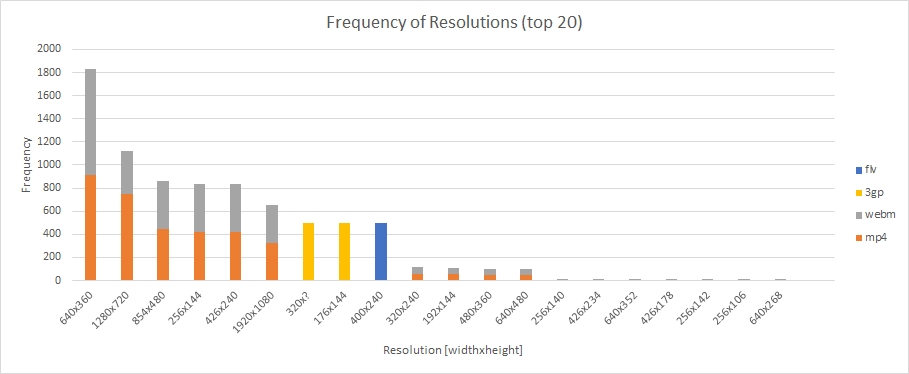
\includegraphics[width=\textwidth]{./frequency-resolution.png}
\caption{Frequency of Resolutions (top 20)}
\label{fig:1}
\end{figure}

\subsection{Analysis of video
bitrates}\label{analysis-of-video-bitrates}

Since the bitrate values where very different (3358 different values) we
assigned the to several bins:

\begin{itemize}
\tightlist
\item
  \textless{}= 64 kbit/s
\item
  65 - 128 kbit/s
\item
  129 - 256 kbit/s
\item
  257 - 512 kbit/s
\item
  513 - 1024 kbit/s
\item
  1025 - 2048 kbit/s
\item
  2049 - 4096 kbit/s
\item
  \textgreater{} 4096 kbit/s
\end{itemize}

For the higher bitrates larger than 4096 kbit/s mainly mp4/avc was used
for videos. For all other lower bitrates mp4/avc and webm/vp9 are nearly
evenly used.

\begin{figure}[htbp]
\centering
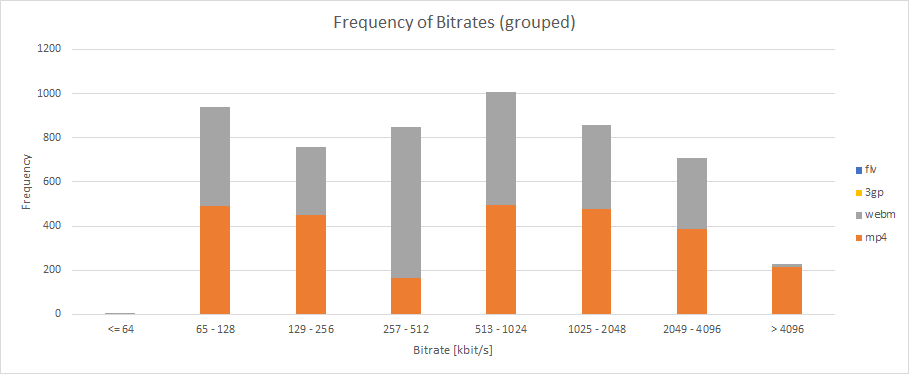
\includegraphics[width=\textwidth]{./frequency-bitrate-cleaned.png}
\caption{Frequency of Bitrates (grouped)}
\label{fig:2}
\end{figure}

\subsection{Number of Representations}

As you can see in figure \ref{fig:3} most of the MPD's contain 12 video representations. They are separated
into two adaptation sets, one for mp4/avc and one for webm/vp9, each containing 6 representations. These
six representations are also the most frequent as shown in figure \ref{fig:1}.

\begin{figure}[htbp]
\centering
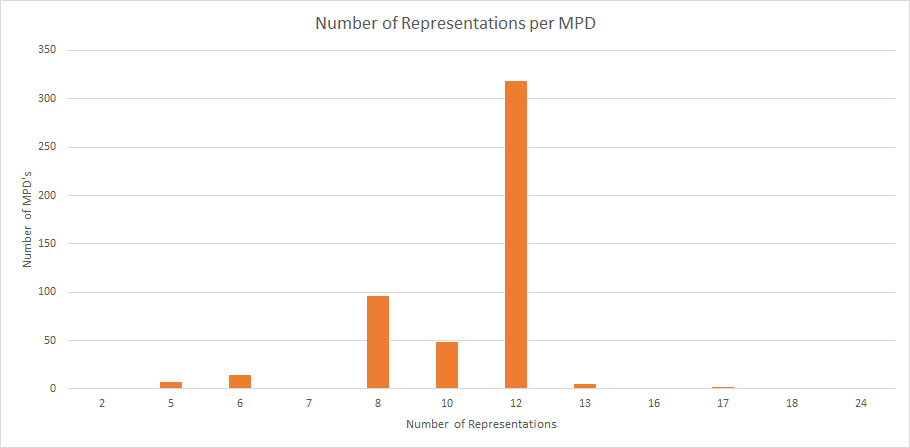
\includegraphics[width=\textwidth]{./number-representations.png}
\caption{Number of Representations per MPD}
\label{fig:3}
\end{figure}


\end{document}
